%%%%%%%%%%%%%%%%%%%%%%%%%%%%%%%%%%%%%%%%%%%%%%%%%%%%%%%%
\documentclass[12pt,a4paper]{article}% 文档格式
\usepackage{ctex,hyperref}% 输出汉字
\usepackage{times}% 英文使用Times New Roman
%%%%%%%%%%%%%%%%%%%%%%%%%%%%%%%%%%%%%%%%%%%%%%%%%%%%%%%%
\title{\fontsize{18pt}{27pt}\selectfont% 小四字号,1.5倍行距
{\heiti% 黑体
Rdrand——基于硬件随机数发生器生成真随机数}}% 题目
%%%%%%%%%%%%%%%%%%%%%%%%%%%%%%%%%%%%%%%%%%%%%%%%%%%%%%%%
\author{\fontsize{12pt}{18pt}\selectfont% 小四字号,1.5倍行距
{\fangsong% 仿宋
白博臣、何骐多、夏营}\\% 标题栏脚注
\fontsize{10.5pt}{15.75pt}\selectfont% 五号字号,1.5倍行距
{\fangsong% 仿宋
(四川大学~~~物理学拔尖计划)}}% 作者单位,“~”表示空格
%%%%%%%%%%%%%%%%%%%%%%%%%%%%%%%%%%%%%%%%%%%%%%%%%%%%%%%%
\date{}% 日期(这里避免生成日期)
%%%%%%%%%%%%%%%%%%%%%%%%%%%%%%%%%%%%%%%%%%%%%%%%%%%%%%%%
\usepackage{amsmath,amsfonts,amssymb}% 为公式输入创造条件的宏包
%%%%%%%%%%%%%%%%%%%%%%%%%%%%%%%%%%%%%%%%%%%%%%%%%%%%%%%%
\usepackage{graphicx}% 图片插入宏包
\usepackage{subfigure}% 并排子图
\usepackage{float}% 浮动环境,用于调整图片位置
\usepackage[export]{adjustbox}% 防止过宽的图片
%%%%%%%%%%%%%%%%%%%%%%%%%%%%%%%%%%%%%%%%%%%%%%%%%%%%%%%%
\usepackage{bibentry}
\usepackage{natbib}% 以上2个为参考文献宏包
%%%%%%%%%%%%%%%%%%%%%%%%%%%%%%%%%%%%%%%%%%%%%%%%%%%%%%%%
\usepackage{abstract}% 两栏文档,一栏摘要及关键字宏包
\renewcommand{\abstracttextfont}{\fangsong}% 摘要内容字体为仿宋
\renewcommand{\abstractname}{\textbf{摘\quad 要}}% 更改摘要二字的样式
%%%%%%%%%%%%%%%%%%%%%%%%%%%%%%%%%%%%%%%%%%%%%%%%%%%%%%%%
\usepackage{xcolor}% 字体颜色宏包
\newcommand{\red}[1]{\textcolor[rgb]{1.00,0.00,0.00}{#1}}
\newcommand{\blue}[1]{\textcolor[rgb]{0.00,0.00,1.00}{#1}}
\newcommand{\green}[1]{\textcolor[rgb]{0.00,1.00,0.00}{#1}}
\newcommand{\darkblue}[1]
{\textcolor[rgb]{0.00,0.00,0.50}{#1}}
\newcommand{\darkgreen}[1]
{\textcolor[rgb]{0.00,0.37,0.00}{#1}}
\newcommand{\darkred}[1]{\textcolor[rgb]{0.60,0.00,0.00}{#1}}
\newcommand{\brown}[1]{\textcolor[rgb]{0.50,0.30,0.00}{#1}}
\newcommand{\purple}[1]{\textcolor[rgb]{0.50,0.00,0.50}{#1}}% 为使用方便而编辑的新指令
%%%%%%%%%%%%%%%%%%%%%%%%%%%%%%%%%%%%%%%%%%%%%%%%%%%%%%%%
\usepackage{url}% 超链接
\usepackage{bm}% 加粗部分公式
\usepackage{multirow}
\usepackage{booktabs}
\usepackage{epstopdf}
\usepackage{epsfig}
\usepackage{longtable}% 长表格
\usepackage{supertabular}% 跨页表格
\usepackage{algorithm}
\usepackage{algorithmic}
\usepackage{changepage}% 换页
%%%%%%%%%%%%%%%%%%%%%%%%%%%%%%%%%%%%%%%%%%%%%%%%%%%%%%%%
\usepackage{enumerate}% 短编号
\usepackage{caption}% 设置标题
\captionsetup[figure]{name=\fontsize{10pt}{15pt}\selectfont Figure}% 设置图片编号头
\captionsetup[table]{name=\fontsize{10pt}{15pt}\selectfont Table}% 设置表格编号头
%%%%%%%%%%%%%%%%%%%%%%%%%%%%%%%%%%%%%%%%%%%%%%%%%%%%%%%%
\usepackage{indentfirst}% 中文首行缩进
\usepackage[left=2.50cm,right=2.50cm,top=2.80cm,bottom=2.50cm]{geometry}% 页边距设置
\renewcommand{\baselinestretch}{1.5}% 定义行间距(1.5)
%%%%%%%%%%%%%%%%%%%%%%%%%%%%%%%%%%%%%%%%%%%%%%%%%%%%%%%%
\usepackage{fancyhdr} %设置全文页眉、页脚的格式
\pagestyle{fancy}
\hypersetup{colorlinks=true,linkcolor=black}% 去除引用红框,改变颜色


%%%%%%%%%%%%%%%%%%%%%%%%%%%%%%%%%%%%%%%%%%%%%%%%%%%%%%%%
\newtheorem{theorem}{\indent 定理}[section]
\newtheorem{lemma}[theorem]{\indent 引理}
\newtheorem{proposition}[theorem]{\indent 命题}
\newtheorem{corollary}[theorem]{\indent 推论}
\newtheorem{definition}{\indent 定义}[section]
\newtheorem{example}{\indent 例}[section]
\newtheorem{remark}{\indent 注}[section]
\newenvironment{solution}{\begin{proof}[\indent\bf 解]}{\end{proof}}
\renewcommand{\proofname}{\indent\bf 证明}

%%%%%%%%%%%%%%%%%%%%%%%%%%%%%%%%%%%%%%%%%%%%%%%%%%%%%%%%

\begin{document}% 以下为正文内容
    \maketitle% 产生标题,没有它无法显示标题
    %%%%%%%%%%%%%%%%%%%%%%%%%%%%%%%%%%%%%%%%%%%%%%%%%%%%%%%%
    \lhead{}% 页眉左边设为空
    \chead{}% 页眉中间设为空
    \rhead{}% 页眉右边设为空
    \lfoot{}% 页脚左边设为空
    \cfoot{\thepage}% 页脚中间显示页码
    \rfoot{}% 页脚右边设为空
    %%%%%%%%%%%%%%%%%%%%%%%%%%%%%%%%%%%%%%%%%%%%%%%%%%%%%%%%
    \begin{figure}[h]
        \centering
        \begin{minipage}{0.32\textwidth}
            \centering
            
\includegraphics[width=\linewidth]{bbc}
            \caption{白博臣}
            \label{fig:img1}
        \end{minipage}\hfill
        \begin{minipage}{0.305\textwidth}
            \centering
            \includegraphics[width=\linewidth]{hqd}
            \caption{何骐多}
            \label{fig:img2}
        \end{minipage}\hfill
        \begin{minipage}{0.32\textwidth}
            \centering
            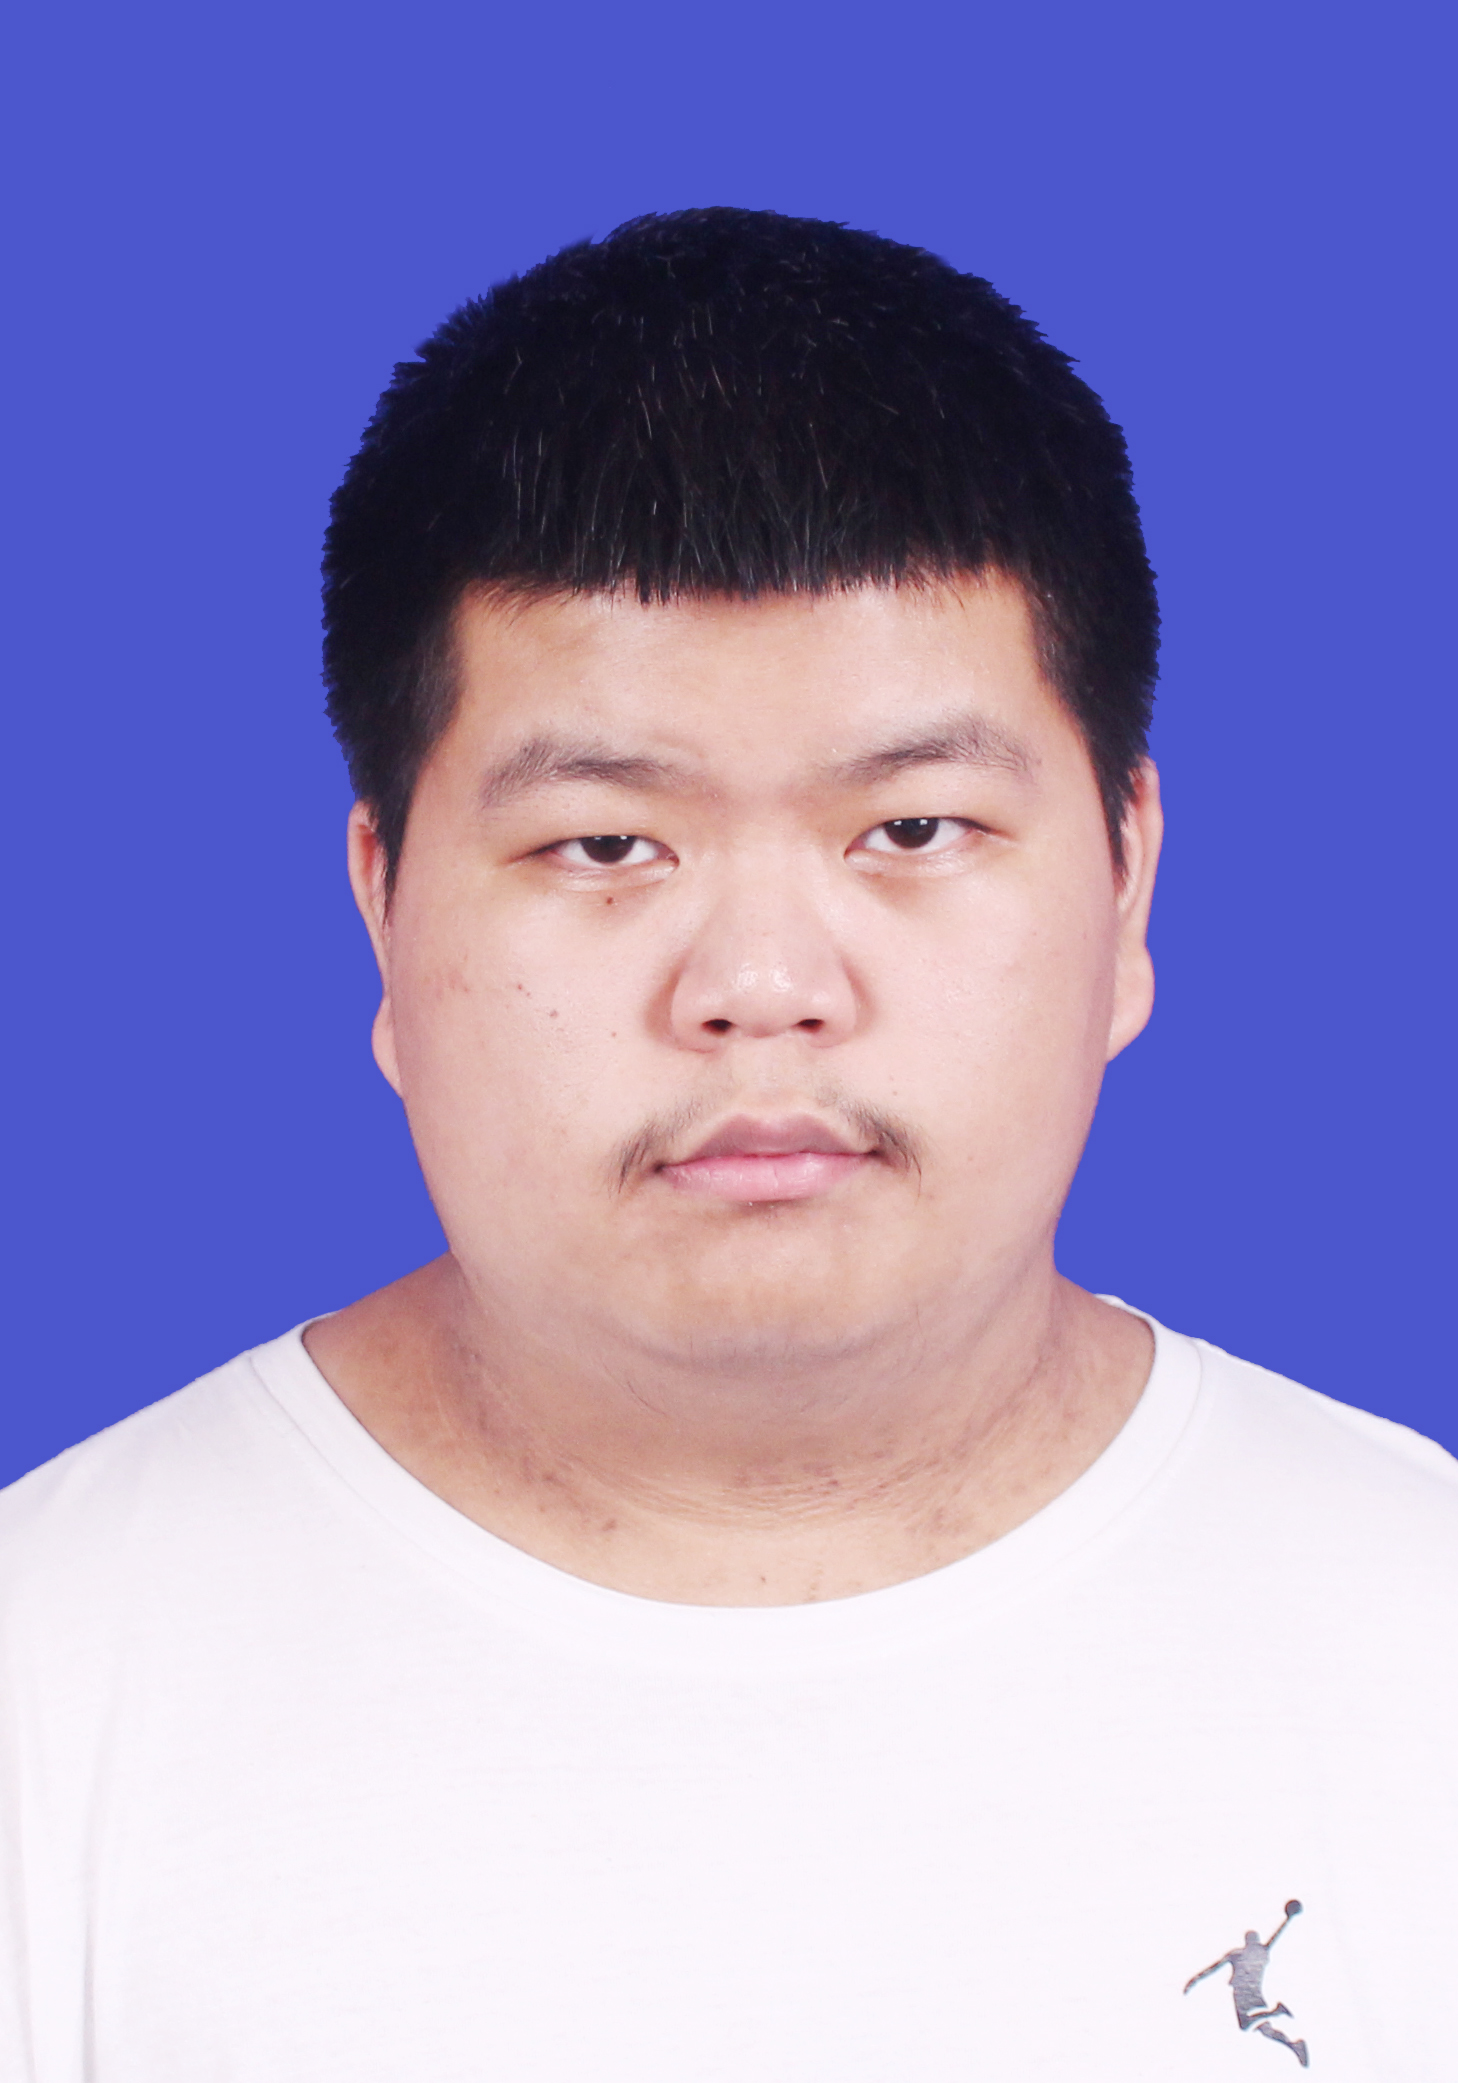
\includegraphics[width=\linewidth]{xy}
            \caption{夏营}
            \label{fig:img3}
        \end{minipage}
    \end{figure}

    \begin{abstract}
        \fangsong
        RDRAND 是一个基于 Intel 芯片实现的利用电阻热噪声实现真随机数生成的一个函数。本文在 \texttt{C/C++, Python, Java} 等语言环境下,基于随机行,均匀性,效率等方向,采用 《GM/T 0005--2021 随机性检测规范》,对该函数进行了测试。讨论了该函数在密码学中的应用,并对其未来进行了展望。

    \end{abstract}

    \begin{adjustwidth}{1.06cm}{1.06cm}
        \fontsize{10.5pt}{15.75pt}\selectfont{\heiti{关键词:}\fangsong{
            RdRand,电阻热噪声,GM/T 0005--2021 随机性检测规范,密码学
        }}\\
    \end{adjustwidth}

%    \begin{center}% 居中处理
%    {\textbf{Abstract}}% 英文摘要
%    \end{center}
%    \begin{adjustwidth}{1.06cm}{1.06cm}% 英文摘要内容
%        \hspace{1.5em}Attention!If you input "dif{}ferent", the computer will output "different", but if you input "dif\{\}ferent", the computer will output "dif{}ferent"
%    \end{adjustwidth}
    \newpage% 从新的一页继续


    \section{引言}
    在蒙特卡洛方法的学习过程中,我们认识到随机数在数值积分中具有极为重要的作用。随机数的随机性质与均匀性质往往会决定计算结果的好坏。目前主流用于计算使用的随机数多是伪随机数与准随机数,这类随机数往往是通过固定的算法或公式产生的序列。其虽然具有较好的随机性质与均匀性质,但这类随机数生成的结果是可预测的,是有规律可循的,故而称为伪随机数或准随机数。而真随机数生成的结果则是完全不可预测的,是真正意义上的“随机”。

    出于兴趣,我们小组对于真随机数进行了一定的探索与研究。在这一过程中,我们发现基于算法直接实现真随机生成比较困难,而一些特定的物理现象本身便具有真随机性,如电阻热噪声、大气噪声等。而Intel正好在其近几年发行的IVB架构的CPU中提供了电阻热噪声的相关数据,于是我们便基于这一硬件提供的电阻热噪声的真随机性实现了真随机数生成器,并基于《GM/T 0005-2021 随机性检测规范》对其随机性质,均匀性质进行了检验,确保我们所得到的随机数是具有良好应用可能性的。


    \section{生成器原理简介}
    电阻的热噪声是其自身产生的噪声,是由导体中电子的振动所引起的,其存在于所有的电子器件与传输介质中。它是温度变化的结果,但不受频率变化的影响。热噪声属于电阻的本征噪声,与外界变量的联系极其微弱。

    噪声产生的源头在于导体中的电子热运动,电子的运动是一种无规则运动,同时因为电子热运动的自由程很短,所以单个电子的运动可以看作产生了一个电流脉冲。而整个导体由热运动所产生的电流,便是导体内所有电子热运动产生电流的叠加,在某一时刻,沿某一方向的热运动可能略占优势,进而产生沿这一方向的电流。但由于电子运动的无规则性,占优势的热运动方向是无法预测的,因而其所带来的噪声具有真随机性。

    而基于电阻热噪声的真随机数生成器便是通过将这个噪声放大,并通过比较器产生二进制随机数序列,是基本没有算法与公式参与的,完全依赖于硬件本身物理性质得到的,产生随机二进制序列的随机数生成器。


    \section{随机性检验}
    因为所得序列为二进制序列,所以可以采用《GM/T 0005-2021 随机性检测规范》给出的15种随机性检验,包括对其随机性、均匀性、自相关性等的检验对所得随机数进行检验,检验方式简介如下:

    \subsection{单比特频数检测方法}
    单比特频数检测是最基本的检测,用来检测一个二元序列中0和1的个数是否相近。随机序列应具有较好的0,1平衡性。在一个足够长的随机序列内,其统计值应服从标准正态分布。

    \subsection{块内频数检测方法}
    块内频数检测用来检测待检序列的$m$位子序列中的1的个数是否接近于$\frac{1}{m}$。对于随机数列而言,其任意长度的子序列中1的个数都应该接近于$\frac{1}{m}$。

    \subsection{扑克检测}
    对任意长度$m$的子序列,其共有$2^m$种不同的组成。对于长度为$N$的待检随机序列而言,将其划分为$[\frac{N}{m}]$(向下取整)个非重叠的长度为m的这$2^m$种子序列出现的个数应当接近。

    \subsection{{重叠子序列检测}}
    扑克检测类似,但是区间划分不同。将长度为$n$的待检序列划分为$n$个可以重叠的长度为m的子序列,在这些子序列中,这$2^m$种出现的个数应当接近。

    \subsection{游程总数检测}
    游程是二元序列的一个子序列,由连续的0或1组成,并且其前导和后继元素都与其本身不同。游程总数检测主要检测待检序列中游程的总数是否服从随机性要求。

    \subsection{游程分布检测}
    连续1(或0)的一个游程称为一个块(或一个间断)。根据Golomb共设,如果待检二元序列是随机的,则相同长度的数目接近一致,且长度为i的游程个数约占总游程个数的$2^{-i}$。

    \subsection{块内最大游程检测}
    将待检序列划分成$N$个等长的子序列,根据各个子序列中最大“1”或“0”游程的分布来评价待检序列的随机性。

    \subsection{二元推导检测}
    二元推导序列是由初始序列生成的一个新的序列。对于长度为n的一个二元初始序列,依次将初始序列中两个相邻比特做异或操作,即可得到该序列的一次二元推导序列,长度为$n-1$。依次执行上述操作$k$次,即可得到k次二元推导序列,长度为$n-k$。二元推导检测的目的是判定第$k$次二元推导序列中0和1的个数是否接近一致。

    \subsection{自相关检测}
    自相关检测用来检测待检序列与将其左移(逻辑左移)$d$位后所得新序列的关联程度。一个随机序列应该和将其左移任意位所得的新序列都是独立的,故其关联程度也应该很低。

    \subsection{矩阵秩检测}
    矩阵秩检测用来检测待检序列中给定长度的子序列之间的线性独立性。由待检序列构造矩阵,然后检测矩阵的行或列之间的线性独立性,矩阵秩的偏移程度可以给出关于线性独立性的量的认识,从而影响对序列随机性好坏的评价。

    \subsection{累加和检测}
    累加和检测将待检序列的各个子序列中最大的偏移(与0之间),也就是最大累加和与一个随机序列应具有的最大偏移相比较,以判断待检序列的最大偏移是过大还是过小。实际上,随机序列的最大偏移应该接近0,所以累加和不能过大,也不能过小(累加和可以是负数)。根据最大偏移值来判断待检序列的随机程度。

    \subsection{近似熵检测}
    近似熵检测通过比较$m$位可重叠子序列模式的频数和$m+1$位可重叠子序列模式的频数来评价其随机性。

    \subsection{线性复杂度检测}
    将待检序列划分为$N$个长度为$m$的子序列,此时$n=N*m$,然后利用Berlekamp-Massey算法(具体内容可网上查询),计算每个子序列的线性复杂度$L_i$,然后利用其给出的统计值来进行随机性判断。

    \subsection{Maurer检测}
    Maurer通用统计(简称通用统计)检测主要检测待检序列能否被无损压缩。如果待检序列能被显著地压缩,则认为该序列是不随机的,因为随机序列是不能被显著压缩的。

    通用统计检测可以用来检测待检序列多方面的特性,但这并不意味着通用统计检测是前面几个检测的拼装,通用统计检测完全采取了和其他检测所不同的方法,可以检测待检序列某些统计上的缺陷。一个序列可以通过通用统计检测当且仅当这个序列是不可压缩的。

    \subsection{离散傅里叶检测}
    离散傅立叶变换检测使用频谱的方法来检测序列的随机性。对待检序列进行傅立叶变换后可以得到尖峰高度,根据随机性的假设,这个尖峰高度不能超过某个门限值(与序列长度$n$有关),否则将其归入不正常的范围;如果不正常的尖峰个数超过了允许值,即可认为待检序列是不随机的。


    \section{随机数检测判定}

    \subsection{样本通过率判定}
    对于每一个随机性检测项目,统计二元序列样本集中$P_{value}$值大于或等于$\alpha$的样本个数,本文确定的用于样本通过率检测的显著性水平$\alpha=0.01$。

    记样本数量为$s$,当通过某检测项目的样本个数大于或等于$s(1-\alpha-3\sqrt{\frac{\alpha(1-\alpha)}{s}})$时,认为该样本集通过该项检测,否则未通过此项检测。例如,样本数量为1000个,则通过该检测项目的样本个数应大于或等于981.

    \subsection{样本分布均匀性判定}
    对于每一个随机性检测项目,二元序列样本集中各样本的$Q_{value}$值应该在区间$[0,1]$均匀分布。记样本数量为$s$,将区间$[0,1]$分为$k$个均匀的子区间,统计二元序列样本集中各样本的$Q_{value}$在$k$个子区间的实际数量$F_i$,并利用$\chi^2$分布与理论值$s/k$进行比较,计算统计值$V=\sum_{i=1}^{k}\frac{(F_i-s/k)^2}{s/k} $,并计算$P_T=igamc(\frac{k-1}{2},\frac{V}{2})$。当$P_T$大于或等于$\alpha_T$时,认为该二元序列样本集通过此项目检测;否则,未通过此项目检测。本文件确定的用于样本分布均匀性检测的显著性水平$\alpha_T=0.0001$,子区间数量$k=10$。


    \section{随机性检测}
    我们不仅对RdRand随机数进行了随机性检测,也对部分主流随机数进行了检测,包括Python中的random库与numpy库的伪随机数,参数为$seed=123, a=1664525, c=1013904223, m=2^32$的LCG以及Matlab中的伪随机数。

    经过随机性检验我们可以发现,Rdrand通过随机性检验的次数要多于另外四种随机数,LCG,Matlab伪随机数和random库伪随机数均出现了不能通过随机性检验的情况,LCG虽然能通过样本通过率判定,但是在分布均匀性上十分糟糕,使用简单的LCG很难得到很好的随机数;Random库伪随机数在块内最大“1”游程检测(m=10000)中没有通过样本通过率判定;Matlab伪随机数没有通过单比特频数检测的样本通过率检测。

    这也反映了Rdrand随机数的优越性,我们可以确保在1000个样本数,每个样本内1000000bit数的情况下,Rdrand随机数的随机性要更加出色,配合原理层面的安全性使其尤其在密码学方向具有自己的独有优势。

    具体结果如下:

    \begin{figure}
        \centering
        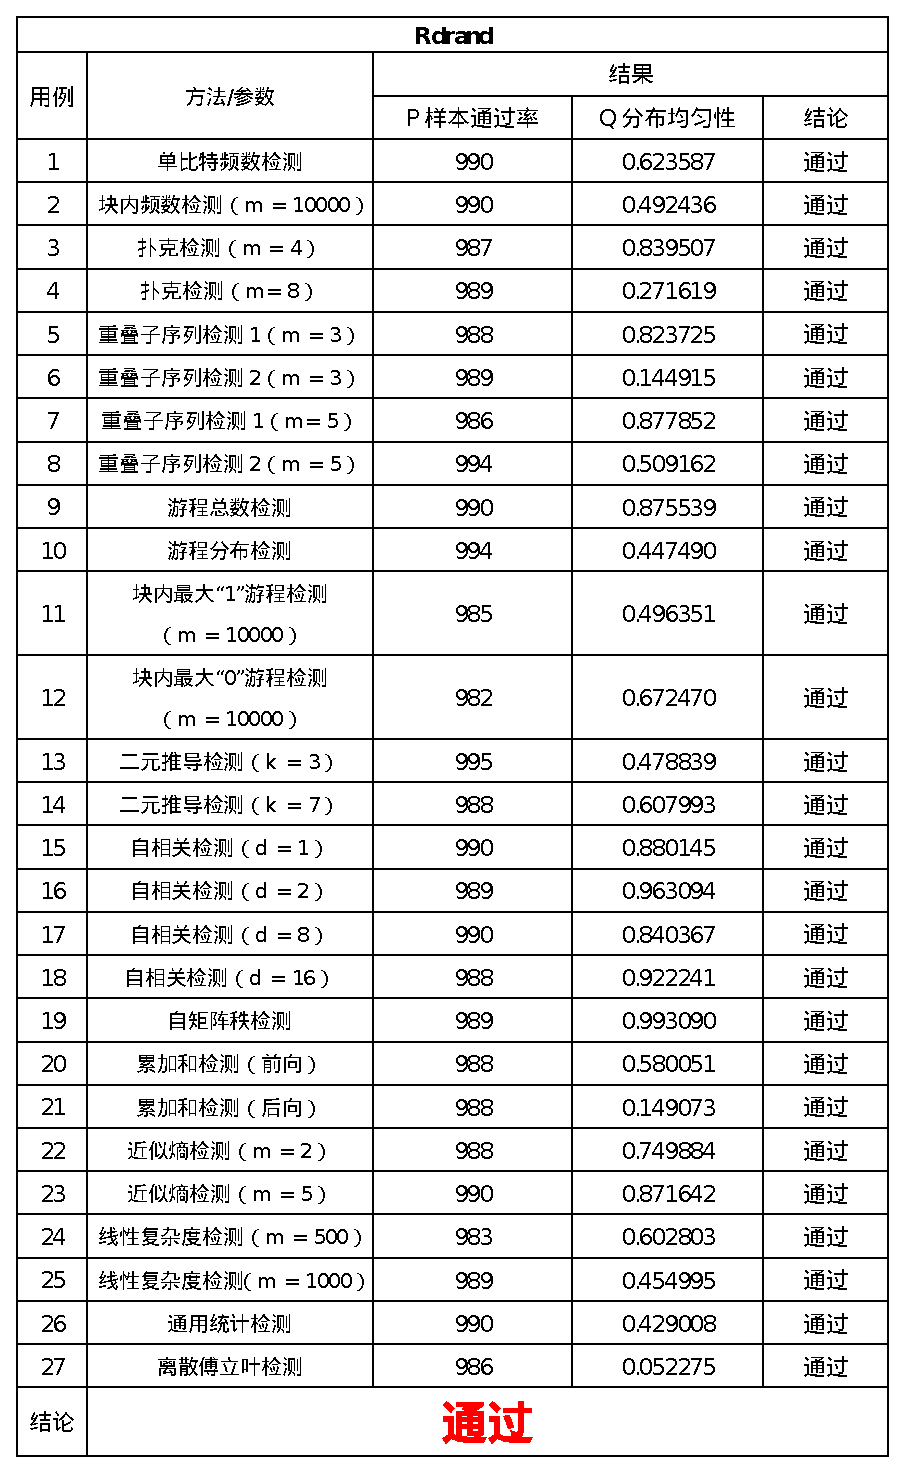
\includegraphics[height=23.7cm]{Rdrand}
        \caption{对RdRand随机数的随机性检验结果}
        \label{fig:fig.1}
        \hypertarget{fig:fig.1}{}

    \end{figure}

    \begin{figure}
        \centering
        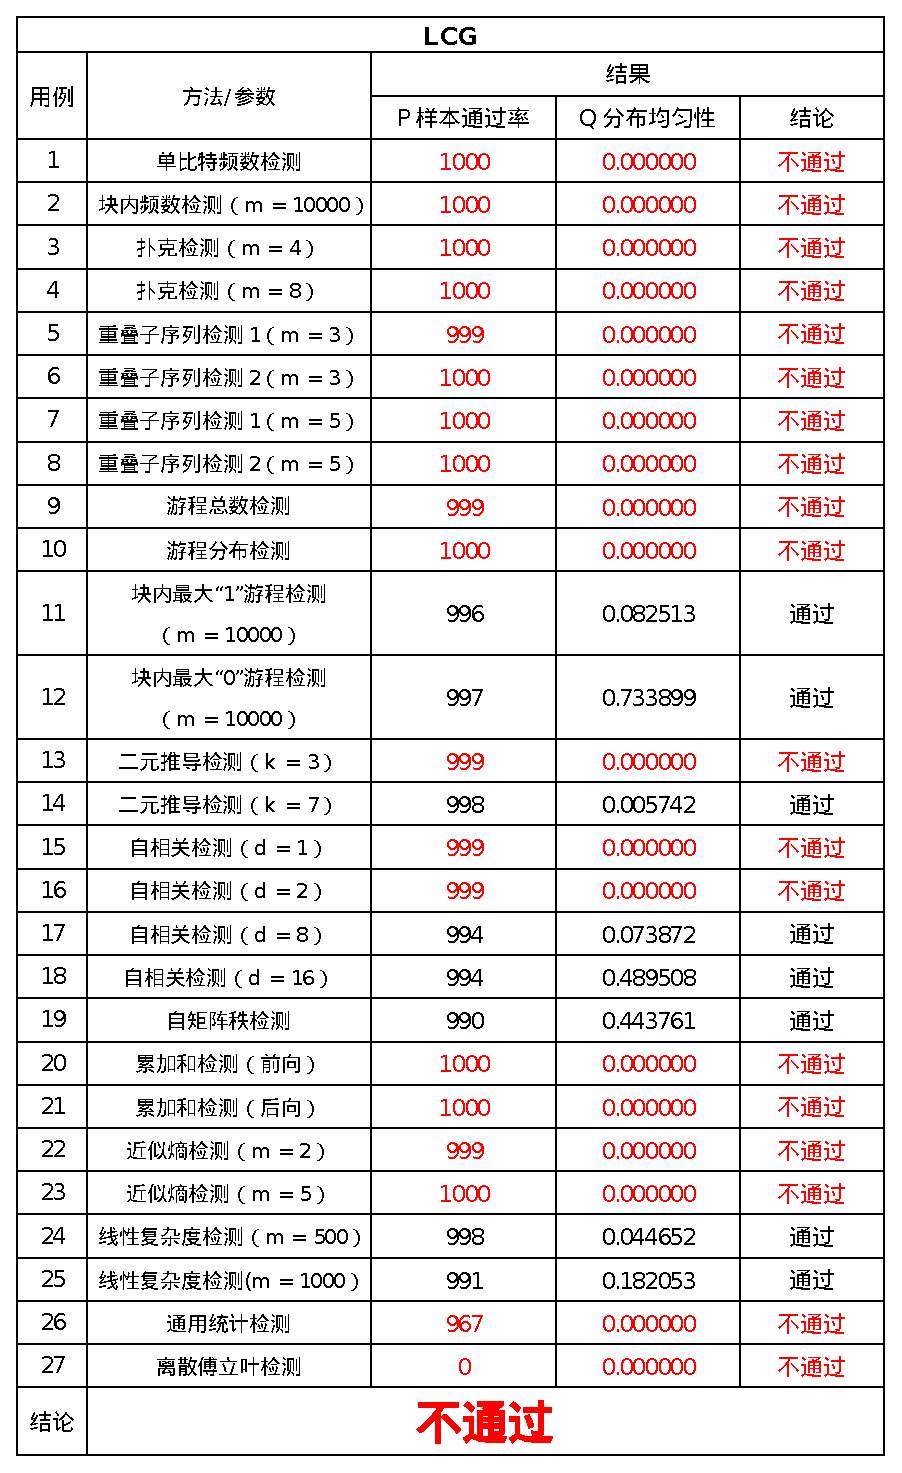
\includegraphics[height=23.7cm]{LCG}
        \caption{对LCG随机数的随机性检验结果}
        \label{fig:fig.2}
        \hypertarget{fig:fig.2}{}

    \end{figure}

    \begin{figure}
        \centering
        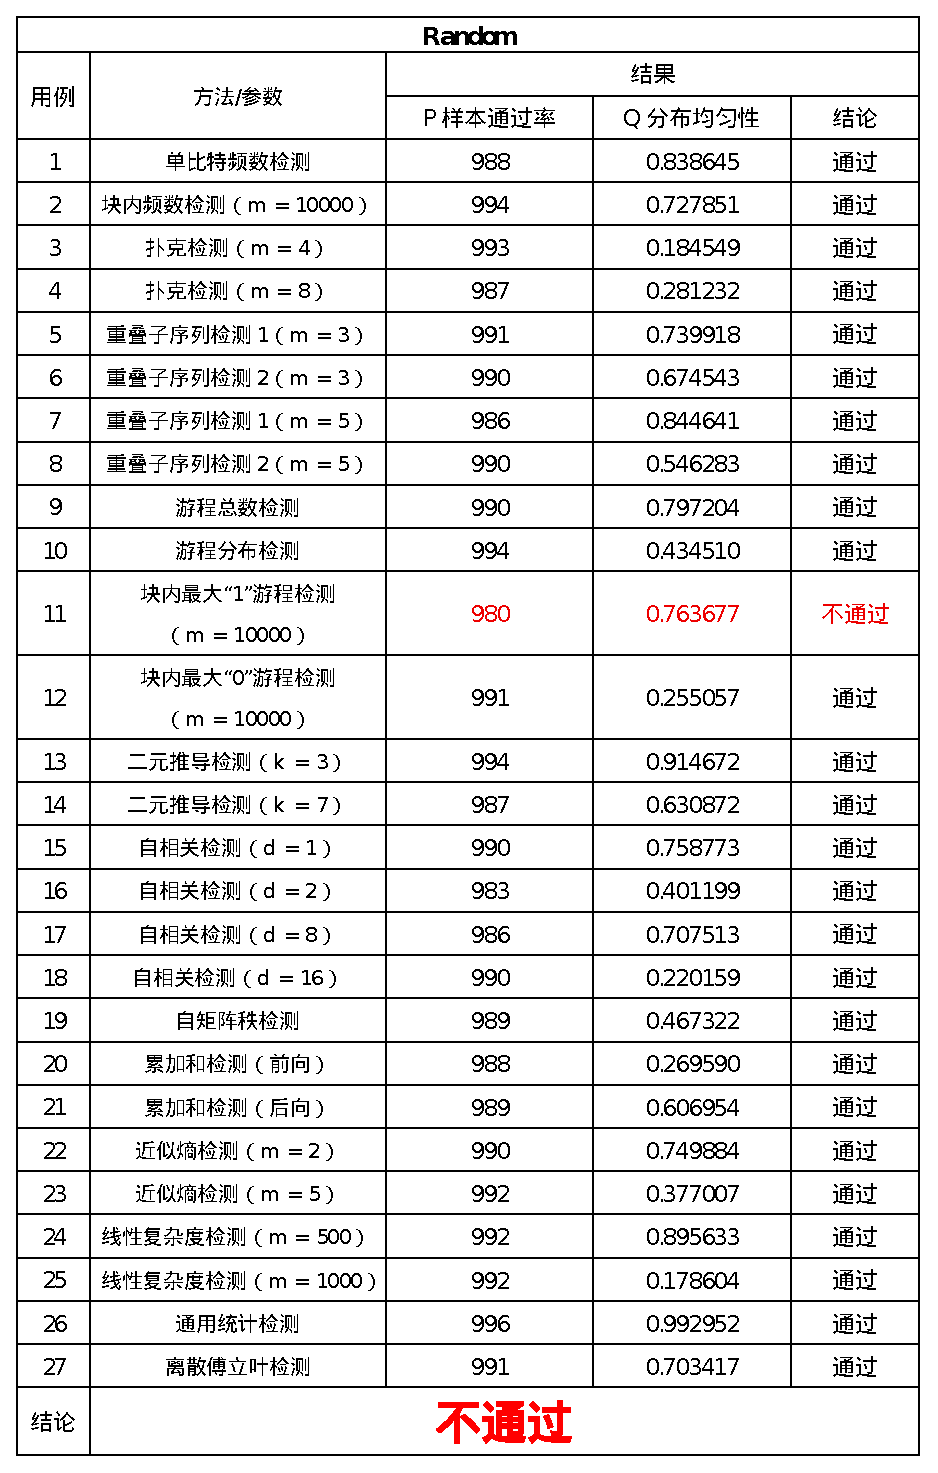
\includegraphics[height=23.7cm]{Random}
        \caption{对random随机数的随机性检验结果}
        \label{fig:fig.3}
        \hypertarget{fig:fig.3}{}

    \end{figure}

    \begin{figure}
        \centering
        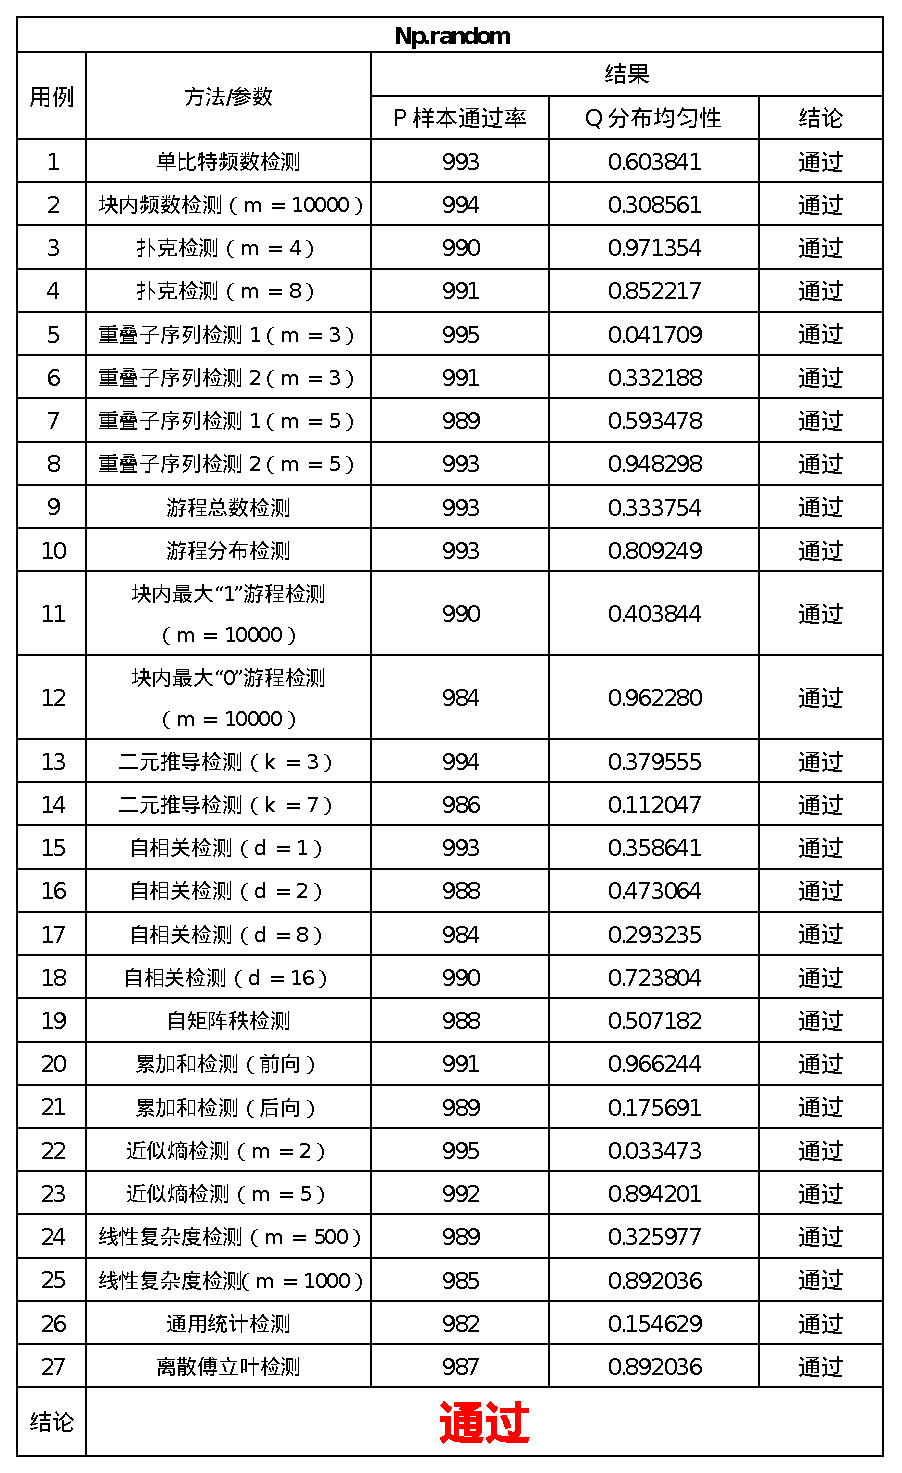
\includegraphics[height=23.7cm]{Np.random}
        \caption{对np.random随机数的随机性检验结果}
        \label{fig:fig.4}
        \hypertarget{fig:fig.4}{}

    \end{figure}

    \begin{figure}
        \centering
        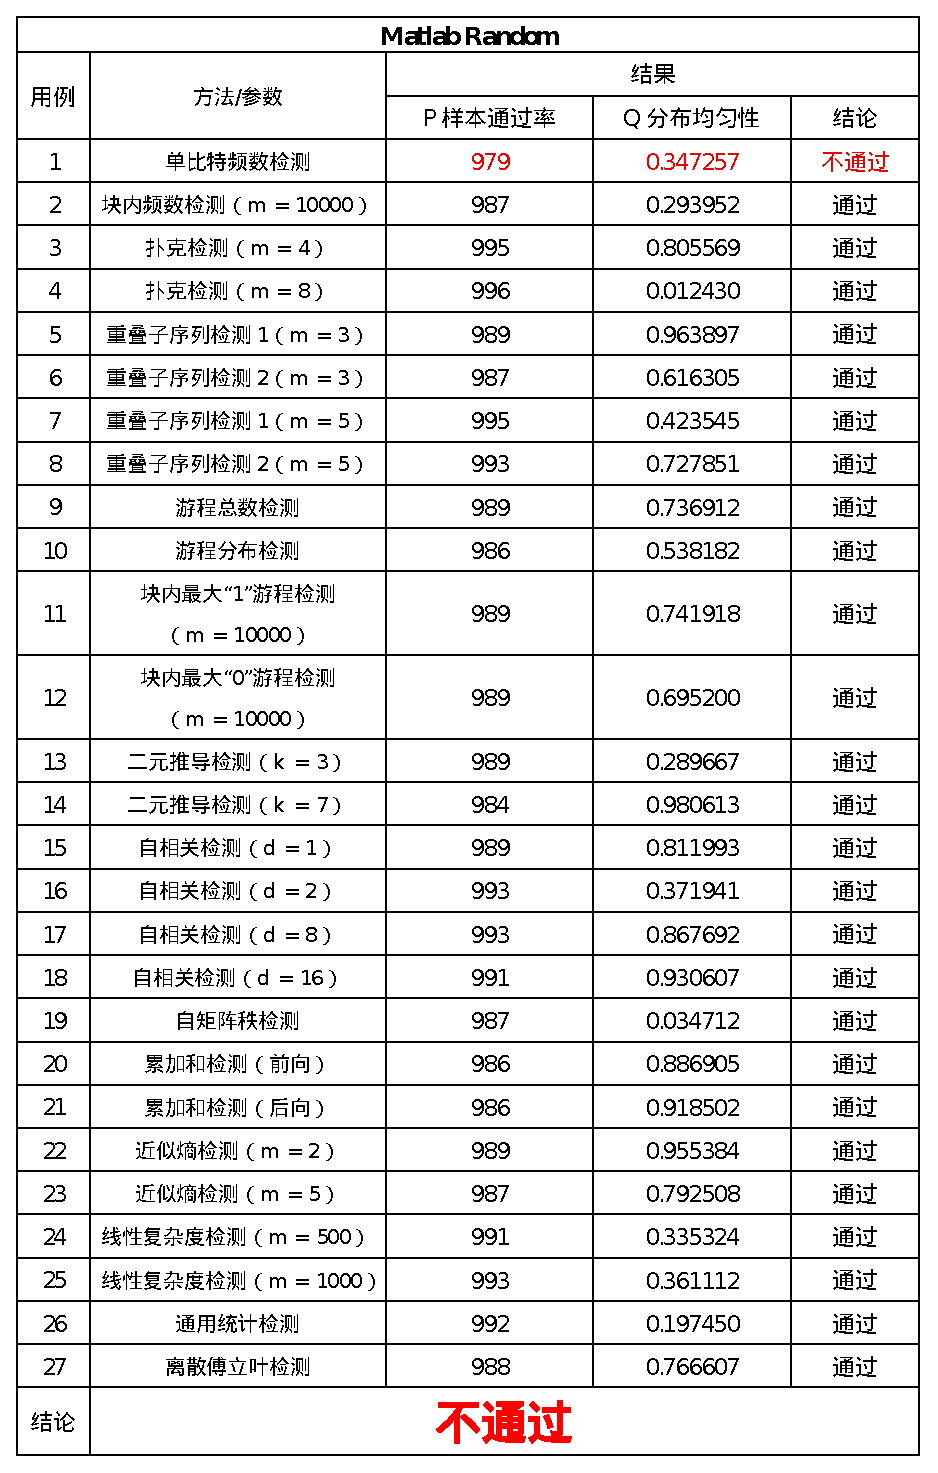
\includegraphics[height=23.7cm]{Matlab random}
        \caption{对Matlab random随机数的随机性检验结果}
        \label{fig:fig.5}
        \hypertarget{fig:fig.5}{}

    \end{figure}
    \newpage


    \section{随机数应用}

    \subsection{随机数效率}
    我们通过测量计算 100 000 个点的运行时间(纳秒值)如下

    \begin{figure}[h]
        \centering
        \includegraphics[height=0.06 \textheight]{speed1}
        \caption{真随机数发生器速度}
    \end{figure}

    对比机器自带伪随机

    \begin{figure}[h]
        \centering
        \includegraphics[height=0.06 \textheight]{speed2}
        \caption{伪随机发生器速度}
    \end{figure}

    牺牲了一定的速度,但换来了更高的随机性,同时其相较于部分其他真随机数生成器在速度上有一定优势。这种随机性带来的难以预测,使得其在安全性上有着较大提升。

    \subsection{具体应用}
    正如前文提到的,这种随机数的诸多性质,决定了其在密码学中具有重要的地位。如今普遍使用的 RSA 体制中,便可使用该随机数进行加密。

    RSA 体制大致阐释如下,用户的数字签名 \(a (0 < a < N - 1)\),通过密钥 \(a^e \equiv b \quad (mod N)\) 进行加密, 收件方收到后,在通过该用户提供的解钥 \(b^d \equiv a \quad (mod N)\) 进行解密。

    使用常规的机器随机数,在大规模的并行计算时,完全有可能出现两条线程使用相同的种子(即系统时有相同的毫秒值),此时生成的随机数便会出现重复,在将其作为密钥加密时,便有可能出现两个不同的用户公用相同的密钥。此时,就会导致即使非该用户的目标对象,也能够得到解钥,从而破解密文。

    在使用 RdRand 时,由于其是基于物理上的混沌系统产生的随机数,其的不可预测性和随机性,保证了不同用户无法截获到其他人的解钥,从而提高了网络传输的安全性。


    \section{总结}
    本文概述了 RdRand 的基本原理,并根据国标《GM/T 0005--2021 随机性检测规范》对该随机数发生其进行了检验。结果说明,RdRand 是具有良好随机性和均匀性的随机数发生器,可以用于实际应用中,例如密码学中。基于其良好的性质,相信在未来,会有更好的发展。


    \section{引言}
    基于先前对于 RdRand 的研究,我们讨论了一个问题,即在 Monte Calo 积分中,不同的随机数生成器的选择,会对收敛阶数造成什么样的影响。

    本文先用概率学的知识,从理论上证明了阶数为 \(O(N^{-1/2})\) 的充分性,在通过代码计算,分析机器的伪随机和 RdRand 的真随机。


    \section{理论推导}
    Monte Calo 方法即一个常规的二项分布,每次进行的 Bernoulli 试验为
    \begin{equation*}
        x =\left\{
        \begin{aligned}
            & 0, \quad The\, point\, is\, out\, of\, the\, area\\
            & 1, \quad The\, point\, is\, in\, the\, area
        \end{aligned}
        \right.
    \end{equation*}

    按照棣莫佛-拉普拉斯定理,二项分布在 \(n\) 足够大时,近似为一个正态分布,有
    \begin{equation*}
        P(\left| \bar{x}_\alpha - I \right| < \frac{\lambda_\alpha \sigma}{\sqrt {N}}) \approx \frac{2}{\sqrt{2 \pi}} \int^{\lambda_\alpha}_0 e^{-\frac{1}{2} t^2} dt = 1 - \alpha
    \end{equation*}
    其中,\(\lambda_\alpha\) 是正态分布的 \(\alpha\) 分位点,\(\sigma\) 是标准差,\(N\) 是试验次数。这表明,不等式
    \begin{equation*}
        \left| \bar{x}_\alpha - I \right| < \frac{\lambda_\alpha \sigma}{\sqrt {N}}
    \end{equation*}
    有置信概率 \(1 - \alpha\) 成立,即 \(\bar{x}_\alpha\) 收敛到 \(I\) 的阶数为 \(O (N^{-1 / 2})\),因此,在后续的实验中应当观察到 \(\ln err - \ln N\) 图中,拟合曲线的斜率为 \(- 1 / 2\)。


    \section{代码验证}
    为了证明以上结果我们分别用 Random 和 RdRand 计算积分 \(\int^1_0 \frac{1}{\sqrt {x} + x} dx\) 的值,观察相对误差随点数 \(N\) 的变化。利用 \texttt{Java} 代码实现,见附件。

    运行结果如下,

    \begin{figure}[h]
        \centering
        \begin{minipage}{0.42\textwidth}
            \centering
            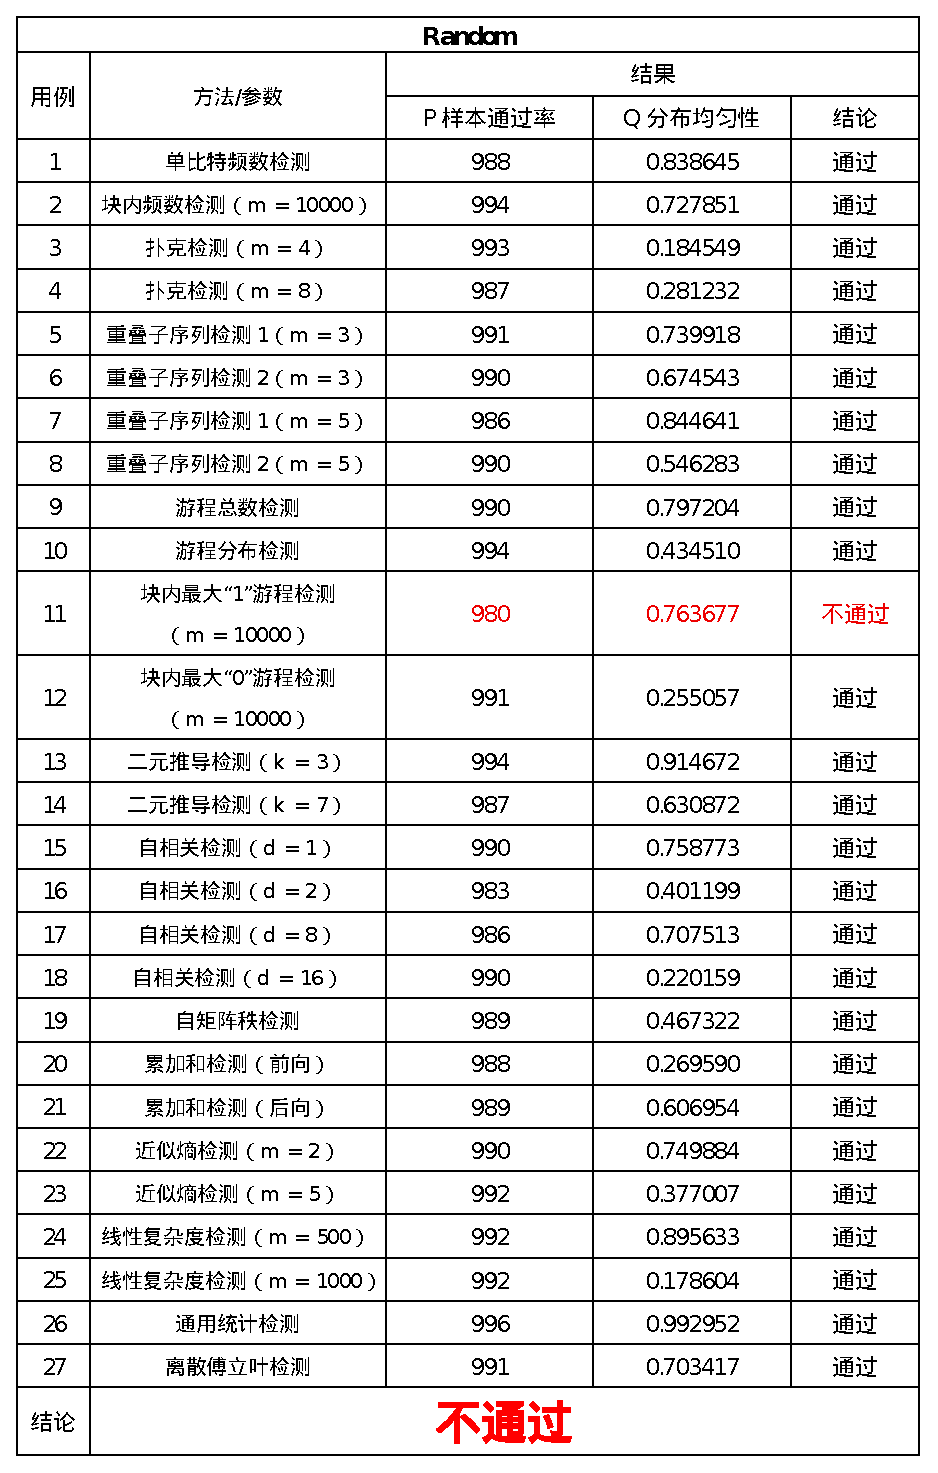
\includegraphics[width=\linewidth]{Random}
            \caption{Random 的运行结果}
            \label{fig:img4}
        \end{minipage}\hfill
        \begin{minipage}{0.42\textwidth}
            \centering
            \includegraphics[width=\linewidth]{RdRand}
            \caption{RdRand 的运行结果}
            \label{fig:img5}
        \end{minipage}\hfill
        \begin{minipage}{0.42\textwidth}
            \centering
            \includegraphics[width=\linewidth]{Random_k}
            \caption{Random 的斜率}
            \label{fig:img6}
        \end{minipage}\hfill
        \begin{minipage}{0.42\textwidth}
            \centering
            \includegraphics[width=\linewidth]{RdRand_k}
            \caption{RdRand 的斜率}
            \label{fig:img7}
        \end{minipage}
    \end{figure}

    \newpage
    由图可见,实验的结果符合理论推导,即在 Monte Calo 积分中,收敛的阶数为 \(O (N^{-1 / 2})\)。


    \section{结论}
    本文通过理论和代码的方式,验证了在 Monte Calo 积分中,收敛的阶数为 \(O (N^{-1 / 2})\),此结论亦可推广到任何 Monte Calo 方法中。不过本文并没有考虑到使用特殊的序列(即准随机),例如 Halton 序列、Sobol 序列和 Niederreiter 序列,这些序列由于其的固定顺序,导致了其并非独立多次的 Bernoulli 试验,无法使用以上理论公式。其在收敛的速度上会更快,斜率的绝对值会更大一些,针对该角度,有待后人更深入的研究。

\end{document}% 结束文档编辑,后面写啥都编译不出来
